%\documentclass{beamer}
\documentclass[handout]{beamer}
\usetheme{boxes} 
%\usetheme{default}

%math fonts
%\renewcommand\mathfamilydefault{\rmdefault}
\usepackage{graphicx}

%page numbers
\setbeamertemplate{footline}[page number]

\setbeamercovered{invisible}
\setbeamertemplate{navigation symbols}{} 
\usepackage{mathtools}
\usepackage{graphicx}
\usepackage{amsmath}
\usepackage{epstopdf}
\usepackage{pgfplots}
\usepackage{color}
\usepackage{subfig}
\usepackage{tikzscale}
\usetikzlibrary{plotmarks}

\title[Trajectory Tracking]{Optimizing Robot Striking Movement Primitives with Iterative Learning Control}
\author{Okan Ko\c c, Guilherme Maeda, Gerhard Neumann, Jan Peters}
\institute[IAS]
{
MPI for Intelligent Systems, T\"ubingen \\
Robot Learning Lab \\
\medskip
{\emph{okan.koc@tuebingen.mpg.de}}
}
\date{\today}

% custom commands
\newcommand{\boldvec}[1]{\boldsymbol{\mathrm{#1}}}
\let\vec\boldvec
\newcommand\at[2]{\left.#1\right|_{#2}} % the at differential sign
\newcommand\scalemath[2]{\scalebox{#1}{\mbox{\ensuremath{\displaystyle #2}}}} % scaling matrices

%% custom macros
\newcommand{\todo}{\textcolor{red}{TODO}} % TODO!
\newcommand{\kin}{\mathcal{T}} % used to denote inverse kinematics
\newcommand{\invKin}{\mathcal{T}^{-1}} % used to denote inverse kinematics

\newcommand{\joint}{\vec{q}} % used to denote robot state in joint space
\newcommand{\state}{\vec{y}} % denotes the generalized coordinates - joint space and velocity coordinates
\newcommand{\dmp}{\vec{s}} % used to denote the dmp trajectory states
\newcommand{\error}{\vec{e}} % difference between state and reference
\newcommand{\traj}{\vec{r}} % used to denote the points on the trajectory to be tracked

\newcommand{\dist}{\vec{\epsilon}} % denotes the disturbances acting on the rigid body dynamics
\newcommand{\linDist}{\vec{d}} % denotes the disturbances on the LTV model

\newcommand{\sysInput}{\vec{u}} % used to denote the system inputs
\newcommand{\linInput}{\tilde{\sysInput}} % denotes the LTV inputs
\newcommand{\trjInput}{\sysInput_{\mathrm{IDM}}} % denotes the inputs on the trajectory (calculated using IDM)


% % % % DMP terminology % % % %
\newcommand{\fullvec}{\vec{\psi}} % full vector for state-ref-dmp-goal
\newcommand{\goal}{\vec{g}} % goal state
\newcommand{\force}{\vec{f}} % forcing term of the dmps
\newcommand{\phase}{x} % phase of the dmp
\newcommand{\weights}{\vec{w}} % weights of the dmp
\newcommand{\basis}{\vec{\Phi}} % basis functions of the dmp as a matrix

% % % % ILC terminology % % % %
\newcommand{\qmatrix}{\vec{\Gamma}} % denotes the filtering qmatrix term of Bristow et al.
\newcommand{\lmatrix}{\vec{L}} % denotes the learning matrix of Bristow et al.

\newcommand{\dynamics}{\vec{f}}
\newcommand{\dynamicsNominal}{\dynamics_{\mathrm{nom}}}
\newcommand{\policy}{\vec{\pi}}
\newcommand{\ValueFunction}{J}
\newcommand{\episode}{k} % used for episode number

\newcommand{\totalTime}{T} % total time duration 
\newcommand{\numSteps}{N} % total number of time steps
\newcommand{\numepisode}{K} % total number of episodes

\newcommand{\threshold}{\epsilon}
\newcommand{\alg}{\emph{wILC }}
\newcommand{\dataset}{E}

% Set the paths where all figures are taken from:
\graphicspath{{Pictures/}}
\mathtoolsset{showonlyrefs} 
\newcommand{\includesvg}[1]{%
% \executeiffilenewer{#1.svg}{#1.pdf}%
% {inkscape -z -D --file=#1.svg %
% --export-pdf=#1.pdf --export-latex}%
 \input{#1.pdf_tex}%
}

\begin{document}
%
\begin{frame}
\titlepage
\end{frame}
%
\begin{frame}
\frametitle{Table of Contents}
\tableofcontents
\end{frame}
%
\section{Motivation}
%
\begin{frame}{Setup}
\begin{itemize}
\item In order to hit the ball to a desired position on the opponent's court, we give the robot reference trajectories that facilitate the right striking motion. We can teach the robot such trajectories via kinesthetic teach-in.
\end{itemize}
\begin{figure}[b!]
\center
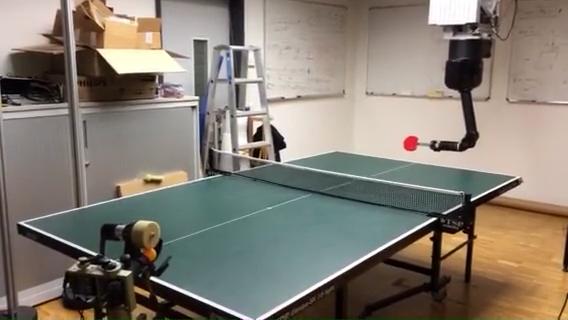
\includegraphics[scale=0.4]{robot1.png}			
\label{robot}
\end{figure}
\end{frame}
%
\begin{frame}{Movement Primitives}
\begin{itemize}
\item Dynamic Movement Primitives (DMP) are a dynamical systems based approach to represent reaching motions:
\begin{equation}
\begin{aligned}
\dot{\dmp} &= \vec{A}_s \dmp + \basis(\phase) \weights \\
\dot{\phase} &= -\tau\alpha\phase.
\label{dmp2}
\end{aligned}
\end{equation}
\item Approximation and control errors in table tennis make the application of DMPs less useful in practice. Small changes to DMPs can often make them more useful.
\end{itemize}
\end{frame}
%
\begin{frame}{Research Question}
\begin{itemize}
\item How can we execute optimally hitting movement primitives either in table tennis or a similar reaching task e.g., putting in golf. 
%
\item More specifically, when we have modelling inaccuracies, how should we modify a DMP $\dmp(t)$ such that the robot executes a desired hitting motion?
\end{itemize}
\end{frame}
%
\begin{frame}{Remark on notation}
\begin{itemize}
\item $k$ denotes the iteration index.
\item $j$ denotes the discretization index.
\item For example $\sysInput_k = [\sysInput_0^{\mathrm{T}}, \ldots, \sysInput_j^{\mathrm{T}}, \ldots, \sysInput_T^{\mathrm{T}}]$ is inputs stacked  together to form a \emph{lifted vector}.
\item Matrices with index $L$ are in accordance with this representation, e.g. \begin{equation*}
\begin{aligned}
 \vec{Q}_L &= 
 \begin{bmatrix}
  \vec{Q}_{1} & \vec{0} & \cdots & \cdots & \vec{0} \\
  \vec{0} & \ddots & \cdots & \cdots & \vdots \\
  \vdots  & \vdots  & \vec{Q}_{j} & \vdots & \vdots \\
  \vdots  & \vdots  & \vdots & \ddots & \vdots \\
  \vec{0} & \cdots & \cdots & \cdots & \vec{Q}_T
 \end{bmatrix}.
\end{aligned}
\end{equation*}
\end{itemize}
\end{frame}
%
\section{ILC on Linear Systems}
%
\begin{frame}{Iterative Learning Control (ILC)}
\begin{itemize}
\item Task: track a reference trajectory $\traj(t), \ 0 \leq t \leq T \ $ under unknown repeating disturbances or model mismatch.
\item Feedforward control inputs $\sysInput(t)$ are adjusted after each iteration. The goal is drive the deviations from the trajectory to zero. 
\end{itemize}
\begin{figure}
\center
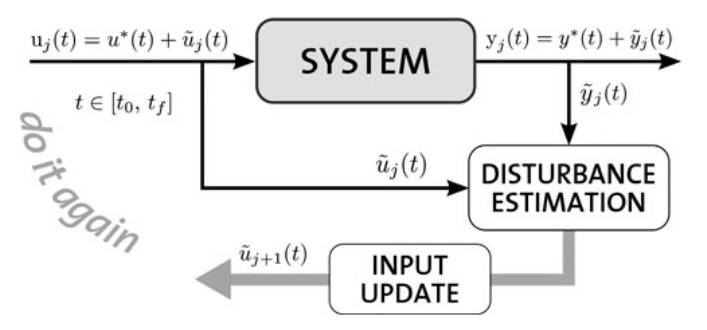
\includegraphics[scale=0.25]{ilc_framework}			
\caption{ILC Framework}
\end{figure}
\end{frame}
%
\begin{frame}{Iterative Learning Control (ILC)}
\begin{itemize}
\item For a linear system $\dot{\state}(t) = \boldvec{A}(t)\state(t) + \boldvec{B}(t)\sysInput(t)$,
\item A very simple update rule is to use the error $\error_k = \state_k - \traj$ and its derivatives. For example:
\begin{equation*}
\begin{aligned}
\sysInput_{k+1} = \sysInput_{k} + K_{p}\error_k + K_{d}\dot{\error}_k
\end{aligned}
\end{equation*}
\item It can easily lead to unstability! Model based update laws can be much more effective in practice!
\end{itemize}
\begin{figure}
\center
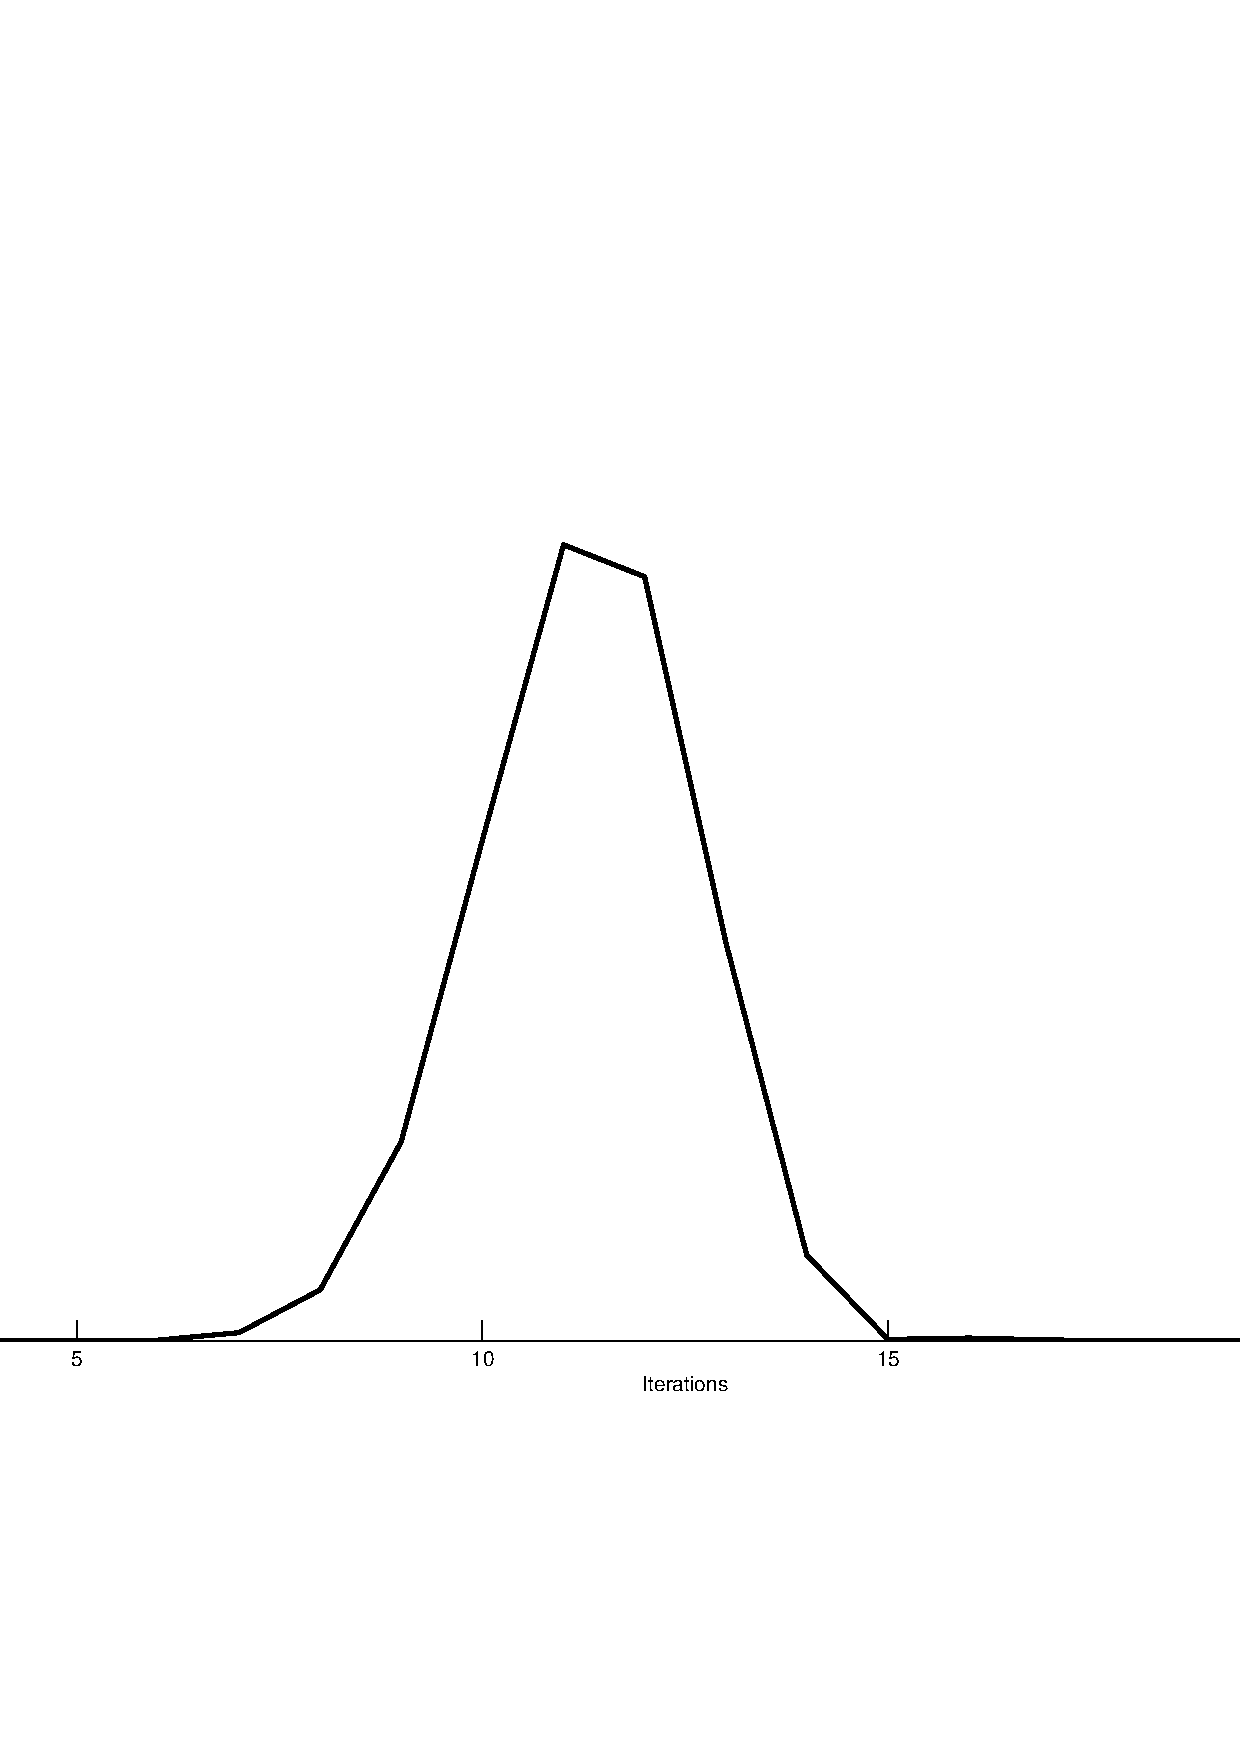
\includegraphics[scale=0.15]{ilcBlowup.pdf}			
\caption{Naive ILC Implementation}
\end{figure}
\end{frame}
%
\begin{frame}{Model-based ILC}
\begin{itemize}
\item ILC update rules can be written generically as: $\sysInput_{k+1} = \qmatrix\sysInput_{k} - \lmatrix\error_{k}$
\item Using the cost functional $\sum_{j=1}^{T} \error_j^{\mathrm{T}}\vec{Q}\error_j + \sysInput_j^{\mathrm{T}}\vec{R}\sysInput_j = \error_k^{\mathrm{T}}\vec{Q}_L\error_k + \sysInput_k^{\mathrm{T}}\vec{R}_L\sysInput_k$ as our optimality criterion,
\item With gradient descent we get: 
\end{itemize}
\begin{equation*}
\begin{aligned}
\qmatrix &= \vec{I} - \beta_k \vec{R}_L \\
\lmatrix &= \vec{F}^{\mathrm{T}}\vec{Q}_L \\
\vec{F}_{(i,j)} &= \left \{
\begin{array}{cc}
\vec{A}_{i-1}\ldots \vec{A}_j\vec{B}_{j-1}, & j < i \\ 
\vec{B}_{j-1}, & j = i \\
\vec{0}, & j > i 
\end{array} \right.
\end{aligned}
\end{equation*}
\end{frame}
%
\begin{frame}{Model-based ILC}
\begin{itemize}
\item $\vec{F}$ is the plant dynamics in the \emph{lifted} domain: $\state_k = \vec{F}\sysInput_k + \linDist_k$
\item With Newton's method 
\begin{equation*}
\begin{aligned}
\lmatrix &= (\vec{F}^{\mathrm{T}}\vec{Q}_L\vec{F} + \vec{R})^{-1}\vec{F}^{\mathrm{T}}\vec{Q}_L \\
\end{aligned}
\end{equation*}
\item Upper diagonal entries of $\lmatrix$ use the model matrices to predict and compensate for the \emph{future} errors on the trajectory. 
\item This noncausal update is very useful for tracking trajectories. What about movement primitives?
\end{itemize}
\end{frame}
%
\section{ILC with DMPs}
%
\begin{frame}{ILC with Movement Primitives}
\begin{itemize}
\item Equivalently we can update the DMP weights $\weights_k$ if we apply feedback $\vec{K}$ on our system
\end{itemize}
\begin{equation*}
\begin{aligned}
\weights_{k+1} &= \weights_{k} - \lmatrix\error_{k} \\
\lmatrix &= (\vec{F}_{w}^{\mathrm{T}}\vec{Q}_L\vec{F}_w + \vec{R})^{-1}\vec{F}_w^{\mathrm{T}}\vec{Q}_L \\
\end{aligned}
\end{equation*}
\begin{itemize}
\item We call this update rule \alg!
\end{itemize}
\begin{figure}
\centering
\def\svgwidth{200pt}
\input{Pictures/fb_plant.pdf_tex}
\caption{Inputs to the feedback coupled system $\vec{P}$ is now $\dmp(t)$.}
\end{figure}
\end{frame}
%
\begin{frame}{ILC with Movement Primitives}
\begin{itemize}
\item $\vec{F}_w$ looks slightly uglier
\end{itemize}
\begin{equation*}
\begin{aligned}
\vec{F}_{w} &= \tilde{\vec{F}}_{w}\vec{F}_{\dmp}\vec{I}_{Nm \times m} \\
(\tilde{\vec{F}}_{w})_{(i,j)} &= \left \{
\begin{array}{cc}
\bar{\vec{A}}_{i}\ldots \bar{\vec{A}}_{j+1}\vec{B}_{j}\vec{K}_{j}, & j < i, \\ 
\vec{B}_{j}\vec{K}_{j}, & j = i, \\
\vec{0}, & j > i,  
\end{array} \right. \\
(\vec{F}_{s})_{(i,j)} &= \left \{
\begin{array}{cc}
\vec{A}_s^{i-1}\basis_{j}, & j < i, \\ 
\basis_{j}, & j = i, \\
\vec{0}, & j > i,  
\end{array} \right. \\
\bar{\vec{A}}_j &= \vec{A}_j - \vec{B}_j\vec{K}_j. \\
\vec{I}_{m\times Nm} &= \begin{bmatrix}
  \vec{I}_{m} & \vec{I}_{m} & \ldots & \vec{I}_{m}
 \end{bmatrix}
\end{aligned}
\end{equation*}

\end{frame}
%
\section{ILC on Nonlinear Systems}
%
\begin{frame}{Learning to Control Robots}
\begin{itemize}
\item Trajectory tracking under the \emph{nonlinear} dynamics of the robot: \pause
\end{itemize}
\begin{equation*}
\begin{aligned}
\ddot{\joint} &= M^{-1}(\joint)\{ \tau - C(\joint,\dot{\joint})\dot{\joint} - G(\joint) \}\\
\ddot{\joint} &= \vec{f}(\joint,\dot{\joint},\sysInput)
\end{aligned}
\end{equation*} \pause
\begin{itemize}
\item Use: An (inaccurate) inverse dynamics model (IDM) of the robot: \pause
\end{itemize}
\begin{equation*}
\begin{aligned}
M(\joint)\ddot{\joint} + C(\joint,\dot{\joint})\dot{\joint} + G(\joint) = \tau \\
\sysInput_{IDM} = \vec{f}_{inv}(\joint_{des},\dot{\joint}_{des},\ddot{\joint}_{des})
\end{aligned}
\end{equation*}
\pause 
\begin{itemize}
\item And a finely-tuned compliant feedback law: \pause
\end{itemize}
\begin{equation*}
\begin{aligned}
\sysInput_{FB} &= -\vec{K}_{p}(\joint - \joint_{des}) - \vec{K}_{d}(\dot{\joint} - \dot{\joint}_{des})
\end{aligned}
\end{equation*}
\end{frame}
%
\begin{frame}{Learning to Control Robots}
\begin{itemize}
\item Linearize the dynamics around the reference trajectory to obtain the time varying matrices $\vec{A}_j, \vec{B}_j$
\end{itemize}
\begin{equation*}
\begin{aligned}
\error_{j+1} &= \vec{A}_j\error_j + \vec{B}_j\sysInput_j + \linDist_j\\
\end{aligned}
\end{equation*} 
\begin{itemize}
\item The time variant matrices are discretizations of 
\end{itemize}
\begin{equation*}
\begin{aligned}
\vec{A}(t) & = \at{\frac{\partial{\mathbf{f}}}{\partial{\state}}}{(\traj(t),\sysInput_{IDM}(t))} \\
\vec{B}(t) & = \at{\frac{\partial{\mathbf{f}}}{\partial{\sysInput}}}{(\traj(t),\sysInput_{IDM}(t))} \\
\end{aligned}
\end{equation*}
\begin{itemize}
\item We use these matrices to construct the learning matrix $L$ for \alg! 
\end{itemize}
\end{frame}
%
\begin{frame}{Toy Example: Putting}
\begin{itemize}
\item Task: follow a pre-assigned trajectory (blue dashed curve) to give the golf ball the right velocity at impact.
\end{itemize}
\begin{figure}[ht]
\centering
\subfloat[Initial attempt]{%
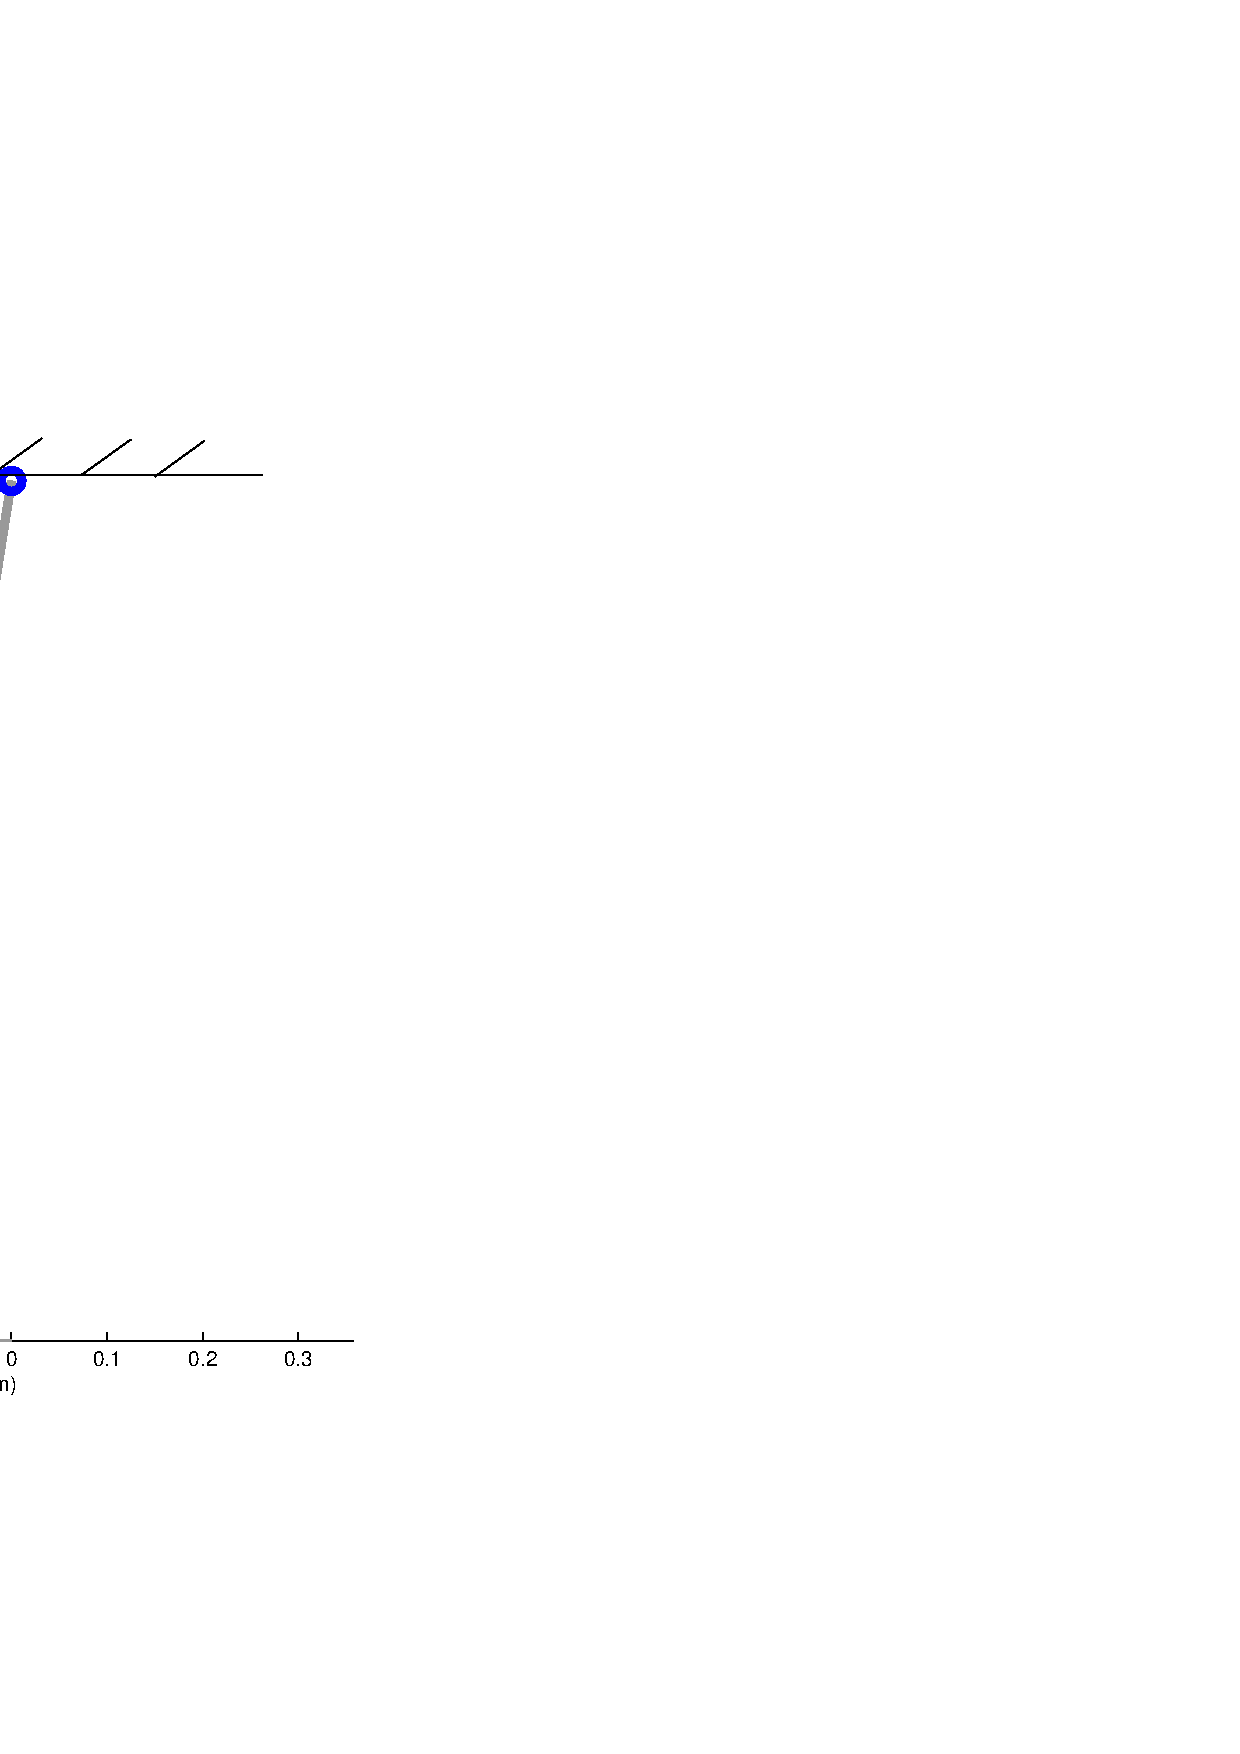
\includegraphics[width=0.3\linewidth]{putting0.pdf}
\label{fig:subfig1}}
\subfloat[Final trajectory]{%
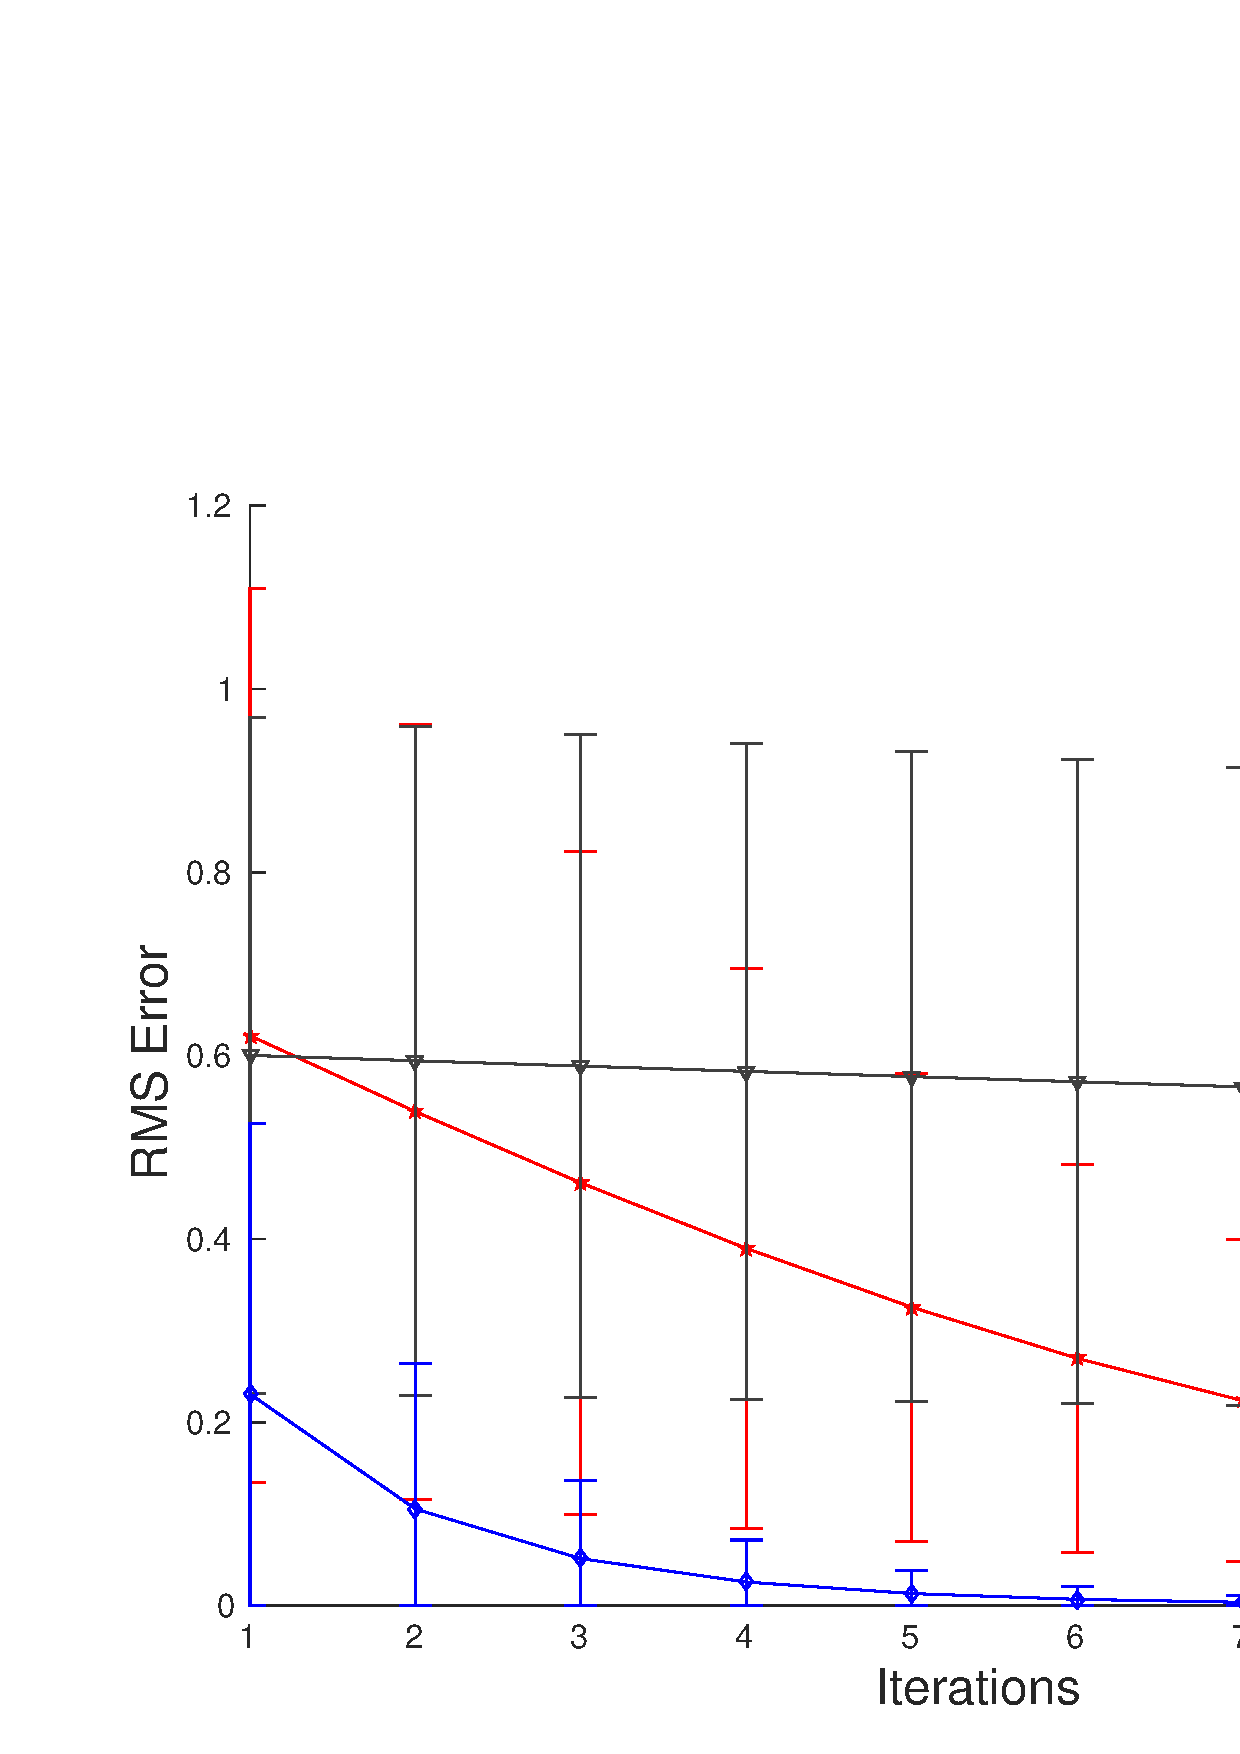
\includegraphics[width=0.3\linewidth]{putting1.pdf}
\label{fig:subfig2}}
\caption{We can see in Fig.~\ref{fig:subfig1} that the initial attempt falls short of the reference trajectory. \alg then modifies the weights of the DMP to compensate for the modeling errors. In Fig.~\ref{fig:subfig2} the reference trajectory is executed perfectly. The ball will then approach the hole, shown as a thick blue line at a distance of 0.5 meters, with approximately zero velocity.} 
\label{putting1} 
\end{figure}
\end{frame}
%
\begin{frame}{Toy Example: Putting}
\begin{figure}
\centering
%\includegraphics[scale=0.50]{comparison.eps}
\newlength\figureheight 
\newlength\figurewidth 
\setlength\figureheight{6cm}  
\setlength\figurewidth{6cm} 
\scalebox{0.8}{% This file was created by matlab2tikz.
% Minimal pgfplots version: 1.9
%
%The latest updates can be retrieved from
%  http://www.mathworks.com/matlabcentral/fileexchange/22022-matlab2tikz
%where you can also make suggestions and rate matlab2tikz.
%
\begin{tikzpicture}

\begin{axis}[%
width=0.95092\figurewidth,
height=\figureheight,
at={(0\figurewidth,0\figureheight)},
scale only axis,
separate axis lines,
every outer x axis line/.append style={black},
every x tick label/.append style={font=\color{black}},
xmin=0,
xmax=12,
xlabel={Iterations},
every outer y axis line/.append style={black},
every y tick label/.append style={font=\color{black}},
ymin=-0.05,
ymax=0.4,
ylabel={RMS Error},
title={Learning Performance in Putting},
legend style={legend cell align=left,align=left,fill=white}
]
\addplot [color=blue,solid]
 plot [error bars/.cd, y dir = both, y explicit]
 table[row sep=crcr, y error plus index=2, y error minus index=3]{%
1	0.233032343134884	0.118115271422138	0.118115271422138\\
2	0.0924719913705091	0.0562589335711811	0.0562589335711811\\
3	0.0384258808828579	0.0276274441478736	0.0276274441478736\\
4	0.0165387503761337	0.0138614543017086	0.0138614543017086\\
5	0.00733384353006482	0.00703352539176592	0.00703352539176592\\
6	0.00333781167932676	0.00358523371207059	0.00358523371207059\\
7	0.00155369907429323	0.0018294817119812	0.0018294817119812\\
8	0.000737146368162867	0.000933121803618784	0.000933121803618784\\
9	0.000355312489801426	0.000475460765776891	0.000475460765776891\\
10	0.000173512604061655	0.000241998267982427	0.000241998267982427\\
};
\addlegendentry{wILC};

\end{axis}
\end{tikzpicture}%}
\caption{Convergence is quadratic for the simulated scenario where we have unknown inertial disturbances acting on the motors.}
\label{wILCTrajectoryPutting}
\end{figure}
\end{frame}
%
\begin{frame}{Recent Developments in the Science of Movement Primitives}
\begin{itemize}
\item Or how to optimally move your primitives!
\item Notice: no matter what weights you choose for $\dmp$, $\dot{\dmp} = \vec{A}_s \dmp + \basis(\phase) \weights$ ensures that you end up at the goal position $\goal$.
\item We don't need to depend on $\traj(t)$ to get to $\goal$: redefining $\error(t) = \state(t) - \dmp(t)$, we can optimize $\error_k^{\mathrm{T}}\vec{Q}_L\error_k + \weights_k^{\mathrm{T}}\vec{R}_L\weights_k$.
\end{itemize}
\end{frame}
%
\begin{frame}{Move Your Primitives}
\begin{itemize}
\item \alg update becomes
\end{itemize}
\begin{equation*}
\begin{aligned}
\weights_{k+1} &= \weights_{k} - \lmatrix_k\error_{k} \\
\lmatrix_k &= (\vec{M}_{k}^{\mathrm{T}}\vec{Q}_L\vec{M}_k + \vec{R})^{-1}\vec{M}_k^{\mathrm{T}}\vec{Q}_L \\
\vec{M}_k &= \vec{F}_{w,k} - \vec{\Psi} \\
\end{aligned}
\end{equation*}
\begin{itemize}
\item $\vec{\Psi}$ comes from the DMP formulation
\end{itemize}
\begin{equation*}
\begin{aligned}
\vec{\Psi} &= \begin{bmatrix}
  \vec{\Phi}_{1} & \vec{0} & \cdots & \vec{0} \\
  \vec{0} & \vec{\Phi}_{2} & \cdots & \vdots \\
  \vdots  & \vdots  & \ddots &  \vdots \\
  \vec{0} & \cdots & \cdots & \vec{\Phi}_T
 \end{bmatrix}.
\end{aligned}
\end{equation*}
\end{frame}
%
\begin{frame}{Future Work}
\begin{itemize}
\item Extensions to the \alg setting: 
\begin{enumerate}
\item Trajectory states are fixed/varying $\checkmark$
\item Time profile is fixed
\item Penalty matrices $\vec{Q},\vec{R}$ are fixed
\item Feedback is fixed
\end{enumerate}
\item For table tennis one needs to consider robust control: ball trajectories may not be well estimated, ball dynamics can be quite wild!
\end{itemize}
\end{frame}
%
\begin{frame}{The End}
\begin{itemize}
\item Thank you for listening!
\end{itemize}
\end{frame}
%
% End of slides
% TODO: add supplementary material!
\begin{frame}{Appendix A: Discretize linearized model}
\begin{itemize}
\item For j $\in \{ 0, 1, \ldots, T-1 \}$, 
\end{itemize}
\begin{equation*}
\begin{aligned}
\error_{j+1} &= \vec{A}_j\error_j + B_j\sysInput_j \\
\end{aligned}
\end{equation*}

\begin{itemize}
\item The discretized matrices can be found using: 
\linebreak
\end{itemize}
\begin{equation*}
\begin{aligned}
\exp^{h
\left[
\scalemath{0.5}{
\begin{array}{c|c}
A(jh) & B(jh) \\ \hline
0 & 0
\end{array}}\right]}
&= 
\left[
\begin{array}{c|c}
\vec{A}_j & \vec{B}_j \\ \hline
0 & I
\end{array}\right]
\end{aligned}
\end{equation*}
\end{frame}
\end{document} 